\documentclass{article}
\usepackage[utf8]{inputenc}
\usepackage{minted}
\usepackage{float}
\usepackage{tikz}
\usetikzlibrary{automata,positioning}

\title{Projet IN406 - Évaluation d’expressions booléennes}
\author{DANKOU Mathis et SOURSOU Adrien}
\date{Mai 2019}

\begin{document}
\maketitle
\section{Questions théoriques}
Question 1:
\vspace{10px}\\*
On définit $G$ la grammaire reconnaissant les expressions booléennes :
\vspace{5px}\\*
\begin{math}
    G = (\Sigma,\;V,\;S,\;P)\\
	\Sigma =\{0,\;1,\;+\;,\;.\;,\;\Rightarrow\;,\;\Leftrightarrow\}\\
    V = \{E,\;C,\;OP\}\\
    S = E\\ 
    P = ( \\
    \hspace*{3ex} E\rightarrow C\;|\;(E)\;|\;NON \;E\;|\;E\;OP\;E \\
    \hspace*{3ex} C\rightarrow \;0\;|\;1 \\
    \hspace*{3ex} OP\rightarrow \;+\;|\;.\;|\;\Rightarrow\;|\;\Leftrightarrow \\
    )
\end{math}
\vspace{10px}
\\*
Question 3:
\vspace{10px}\\*
c = $[\;[\;NON\;|\;(^*\;]^*\;[\;0\;|\;1\;]\;)^*$ \\
e = $c\;[\;[\;+\;|\;.\;|\;\Rightarrow\;|\;\Leftrightarrow\;]\;c\;]^*$ \\
On définit le langage $L$, tel que $L = \{\; w \in e,\; n\; \geq 0,\; |w|_{(} = |w|_{)} = n\;\}$
\begin{figure}[H]
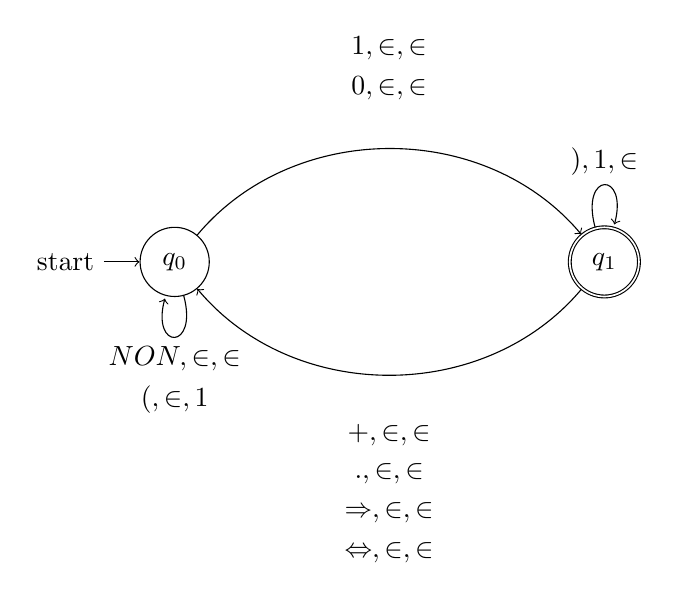
\begin{tikzpicture}
   \node[state,initial] (q_0)  {$q_0$}; 
   \node[state, accepting] (q_1) [right=5cm] {$q_1$}; 
    \path[->] 
    (q_0)   edge [loop below] node[below=0.0] {$NON,\in,\in$}
                              node[below=0.5] {$(,\in,1$} ()
            edge [bend left=50] node[above=1] {$1,\in,\in$}
                                node[above=0.5] {$0,\in,\in$} (q_1)
    (q_1)   edge [loop above] node {$),1,\in$} ()
            edge [bend left=50] node[below=0.5] {$+,\in,\in$}
                                node[below=1] {$.,\in,\in$}
                                node[below=1.5] {$\Rightarrow,\in,\in$}
                                node[below=2] {$\Leftrightarrow,\in,\in$} (q_0);

\end{tikzpicture}
\caption{Automate à pile reconnaissant le langage par état final et pile vide.}
\end{figure}
\noindent Question 7:
\vspace{10px}\\*
La priorité des opérateurs est décrite par le tableau de priorité ci-dessous:
\vspace{5px}

\begin{tabular}[h]{|r|l|}
\hline 
    Opérateur & Priorité\\ 
\hline 
    NON & 1\\
\hline 
    . & 2\\
\hline 
    + & 3\\
\hline 
    $\Rightarrow$ & 4\\
\hline 
    $\Leftrightarrow$ & 5\\
\hline
\end{tabular}
\section{Commentaires}
\begin{minted}{C}
typedef struct token* liste_token;
struct token
{
	e_type type;
	e_valeur valeur;
	liste_token suivant;
};

typedef struct arbre* arbre_token;
struct arbre
{
	e_type type;
	e_valeur valeur;
	arbre_token gauche;
	arbre_token droite;
};
\end{minted}
Le programme par défaut n'affiche que le résultat de l'expression, une variable DEBUG peut être modifiée afin de visualiser l'arbre construit.\\
En plus des fonctions \textit{string\_to\_token} et \textit{arbre\_to\_int}, nous utilisons la fonction \textit{liste\_token\_to\_postfixe}, permettant de transformer notre liste de tokens en liste postfixe.
Au sein de la fonction \textit{arbre\_to\_int}, les éléments de type constante de la liste sont ajoutés à un tableau d'arbre\_token servant de pile. Les arbres sont combinés ensemble lorsque un token avec le type opérateur est rencontré. 
\\
La conversion de la chaîne de caractère en liste de tokens se fait en un seul parcours.
La liste de tokens est parcourue à trois reprise: une première fois afin de la transformer en liste de tokens postfixe, une seconde afin de calculer la taille maximum de notre pile d'arbres et une dernière fois pour construire notre arbre de tokens.\\
On peut ainsi estimer que la complexité de notre programme est en $O(n)$ linéaire.
\end{document}
